\documentclass[11pt]{article}
\usepackage[margin=1in]{geometry}
\usepackage[T1]{fontenc}
\usepackage{lmodern,microtype,booktabs,graphicx,amsmath,xurl}
\usepackage[hidelinks]{hyperref}
\newcommand{\vattempts}{5}
\newcommand{\vclaims}{5}
\newcommand{\vsurvived}{5}
\newcommand{\vclaimlo}{0.57}
\newcommand{\vclaimhi}{1.00}
\newcommand{\vattemptsurvived}{5}
\newcommand{\vattemptlo}{0.57}
\newcommand{\vattempthi}{1.00}
\newcommand{\vrecords}{4}
\newcommand{\vshrink}{1.00}
\newcommand{\vbestgain}{0.0188}
\newcommand{\vseedrunslo}{8}
\newcommand{\vseedrunshi}{44}
\newcommand{\vcostlo}{2.21}
\newcommand{\vcosthi}{4.49}
\newcommand{\vnullrecords}{3}
\newcommand{\vnullfalse}{0}
\newcommand{\vnulln}{24}
\newcommand{\vnullrefuted}{1}
\newcommand{\vfairmachines}{?}
\newcommand{\vfairmax}{?}
\newcommand{\vfairratio}{?}
\newcommand{\vfairseeds}{?}
\newcommand{\vtolerance}{?}
\newcommand{\vfairp}{?}
\newcommand{\vfairentry}{?}
\newcommand{\vfairreference}{?}
\newcommand{\vquickseconds}{?}
\newcommand{\vquickrun}{https://github.com/abhaymettu/odometer}
\newcommand{\vattacks}{79}
\newcommand{\vrecordtest}{1.0976}
\newcommand{\vrecordname}{Mixing, words and story boundaries}

\title{odometer: a training speedrun metered per operation, with coding agents on the record table}
\author{Abhay Mettu\\\small\url{https://github.com/abhaymettu/odometer}}
\date{}
\begin{document}
\maketitle

\begin{abstract}
Training speedruns score wall-clock time, so a record measures the idea and the hardware together and a number from one machine means little on another. odometer replaces the clock with a meter. Every tensor operation costs ticks, priced from its shape alone and calibrated to be close to time, and an entry gets $4\times10^{10}$ ticks to train a byte-level model on TinyStories. The same program reaches the same reading on every machine: across \vfairmachines{} machines tick counts were identical and held-out scores differed by at most \vfairmax{} bits per byte, about \vfairratio{} times below the margin a record has to clear. A verifier small enough to read reruns each entry on fresh seeds on a held-out split, and \vattacks{} entries written to cheat pin how it fails and where it still has holes. On this track I ran a preregistered series of \vattempts{} isolated Claude Code sessions. \vrecords{} of \vclaims{} claims cleared the record rule after a written review. All \vsurvived{} replicated on fresh seeds, a count that could hardly have come out otherwise, since dev and test are a random split of one file. The nearest precedent, a public leaderboard that ranks estimators on metered FLOPs, meters estimation and not training, and I found no public record track that meters the training run itself.
\end{abstract}

\section{The problem with a clock}
A training speedrun needs a budget, and every common budget has a problem. Wall-clock limits tie results to hardware, as the README of karpathy/autoresearch says of its own five-minute runs, which ``become not comparable to other people running on other compute platforms''. Standardized hardware fixes comparability at the price of access: modded-nanogpt and OpenAI's Parameter Golf run on eight H100s, and MLCommons AlgoPerf fixes its own accelerators. A step count, as in modded-nanogpt's optimization track, is free of hardware but only works with the model held fixed.

The obvious replacement, counting floating-point operations, has a problem for training. Calibrated to time, a matmul costs one tick per 128 multiply-adds and \texttt{exp} one tick per element, so under a flat FLOP price an entry heavy on elementwise work would take about a hundred times longer for the same reading, and an agent would find that gap quickly. odometer prices operations close to their real cost instead, from shapes alone, so that the reading depends only on the program for any program that does not branch on its floats, and no entry is much slower than its reading suggests.

\section{The track}
An entry is one Python file with \texttt{train(data)} and \texttt{forward(params, x)}, written against a small tensor engine with reverse-mode gradients. Each call advances one global odometer. A tick is about one nanosecond of one laptop core. Prices depend only on shapes: for example, a matmul of $(m,k)$ by $(k,n)$ costs $\max(m,8)\max(k,64)\max(n,8)/128$ plus a constant per batch element, cheap elementwise work costs one tick per four elements, and \texttt{exp} and \texttt{log} cost one tick per element. When a charge would pass the budget, the operation raises and every later operation raises too.

The score is held-out bits per byte on 1024 windows of 512 bytes from TinyStories V2 \cite{tinystories}, split at random into a dev pool and a test pool. One seed of a record takes about \vtwolo{} to \vtwohi{} seconds on a 2-core CI runner, so a record can be checked at home. The number of bytes read, the model family and the optimizer are all the entry's choice.

Prices are close to time and not equal to it. Against the median, 331 of 335 calibration rows on x86 sit within a factor of 5. A copying \texttt{reshape} and its backward run about 7 times over their price, and squaring and \texttt{embedding} run about 6 to 7 times under theirs. Prices were frozen once records stood on them, so a misprice is disclosed and not fixed, and any later change would need a new version of the track and a new table.

\section{Same program, same reading}
Ticks must match exactly across machines. Scores pass through each machine's BLAS, so they may differ in the last digits. The same \vfairseeds{} seeds of the current record ran on each machine, and each was compared with a reference by a paired equivalence test (TOST) against a tolerance of $\pm\vtolerance$ bits per byte, fixed before the machines ran. \vbranchnote{} Table~\ref{tab:fair} is generated from the logs.

\begin{table}[h]\centering\small
\begin{tabular}{lcccc}
\toprule
Machine & Same seeds & Ticks identical & Largest difference, bits per byte & Paired TOST p \\
\midrule
Linux aarch64, 4 cores, scipy-openblas 0.3.34.106.0 & 4 & yes & 1.3e-08 & 1.5e-13 \\
macOS arm64, 3 cores, accelerate & 4 & yes & 4.2e-08 & 3.5e-12 \\
macOS x86\_64, 4 cores, accelerate & 4 & yes & 3.5e-08 & 9.8e-13 \\
Linux x86\_64 on a Ryzen 9700X VM, 4 cores, scipy-openblas 0.3.34.106.0 & 4 & yes & 2.9e-08 & 6.8e-13 \\
\bottomrule
\end{tabular}

\caption{The same seeds of the current record, each machine against the reference (\vfairreference). Ticks are train and eval ticks per byte.}\label{tab:fair}
\end{table}

The demo on the project page runs the current record's unchanged code in a browser under Pyodide at a smaller budget, and it stopped at the same tick as native code. Its purpose is to show the property directly, and it is not a score.

\section{What a rerun guarantees}
\texttt{verify.py} is the referee. Training runs in its own process, which never loads held-out bytes, and scoring runs in a second, fresh one. Static rules limit an entry's imports to \texttt{odometer} and \texttt{math}, restrict the names it can use, and ration literals and syntax nodes so that a table cannot travel in the source. Python work outside the engine is counted in lines, and training reads through \texttt{item()} are rationed. A quarter of the scored windows have a twin that shares a prefix and differs after a random cut, and if the logits before the cut move, the entry was looking ahead or across rows and the run is void.

A new record has to beat the holder by more than 0.002 bits per byte at one-sided Welch $p<0.01$ on 8 fresh seeds, repeat that on 8 new seeds, and then get a written review that explains what buys the gain. Stored incumbent numbers are 8 further fresh seeds that played no part in seating that record, and later claims are compared with them.

The test suite holds \vattacks{} entries written to cheat: reading held-out bytes, looking ahead, keeping state between calls, getting compute for free, shipping data in the source, and breaking the verifier. A test pins the exact way each fails. Four still work, and they are pinned too. Three obtain compute for free: \texttt{sum(range(n))} is one counted line, Python big integers do vector arithmetic for almost no ticks, and a line of 2000 additions counts once. With only 20,000 reads of training data, that compute has little to learn from, which is inferred and not measured. The fourth is a look-ahead bonus under the twin tolerance, worth under $1.5\times10^{-4}$ bits per byte. There is no memory or disk cap. The test split is public to entrants, so a record rests on published logs and a review and not on a seal. The obvious attack is a table of test text in the source: the 4096-byte literal cap allows 32,768 bits against 524,288 scored bytes, a ceiling of 0.0625 bits per byte, 31 times the margin. How much of that a real table gets is unmeasured.

\begin{figure}[t]\centering
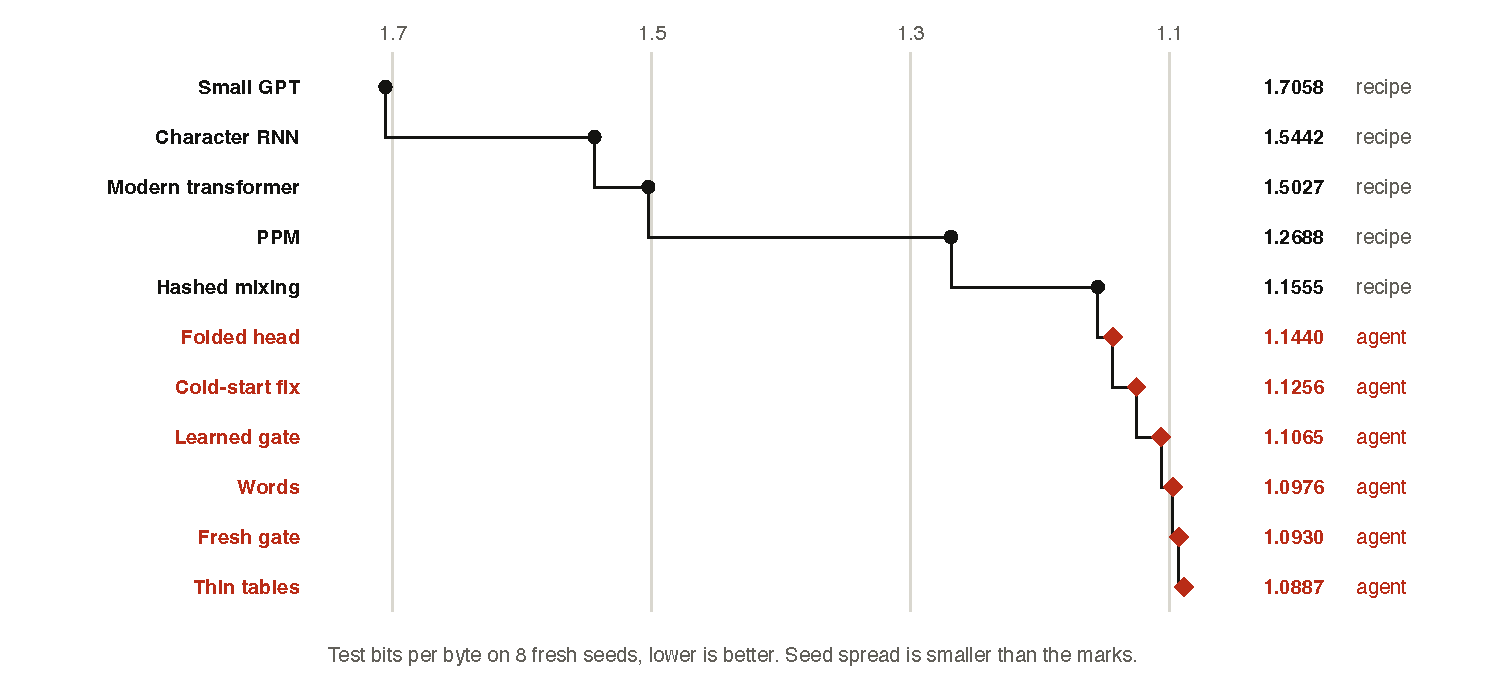
\includegraphics[width=\linewidth]{fig/ladder.pdf}
\caption{The record table. Circles are recipes ported from the literature and tuned on dev, and diamonds are agent entries. No person has run this track, so the recipes are baselines and not human records.}\label{fig:ladder}
\end{figure}

\section{An agent series}
\paragraph{Design.} The plan, the count and the classification rule were committed before the first counted attempt (\texttt{study/PREREG.md}). Each attempt gave one Claude Code session Opus 5.5 at high effort, 40 minutes on a 4-core VM, and the current record to start from, in a filesystem view with an empty home, no user configuration, and a copy of the held-out data with every byte outside dev windows zeroed. It kept web access. The agent could write up to 3 claims. After it exited, each claim was rerun in CI on 8 fresh seeds on the test split. A claim is \emph{replicated} if the one-sided $p$ that the gain is positive is below 0.01, \emph{refuted} if not replicated and the interval's upper bound is below the claimed gain, \emph{rejected} if the verifier voids it, and otherwise \emph{inconclusive}. Attempts ran in sequence, and a seated record became the next starting point. Two pilots ran before registration and are reported apart. They changed the model, the allowance and the prompt's last line.

\paragraph{Results.} \vrecords{} of \vclaims{} claims cleared the record rule, with gains falling from \vbestgain{} to \vgainlast{} bits per byte. All \vsurvived{} replicated (Wilson 95\% interval \vclaimlo{} to \vclaimhi), and \vattemptsurvived{} of \vattempts{} attempts had a replicated claim (\vattemptlo{} to \vattempthi). That count could hardly have come out otherwise: dev and test are a random split of one file, and in simulation, had every claim been exact, all \vclaims{} replicate with probability above 0.999, and at half the claimed gain still about \vphalf{}. It mainly rules out a broken pipeline or misreported dev means. The registered shrinkage hypothesis cannot be resolved at this size: the median of verified over claimed gain was \vshrink{}, with \vshrinkbelow{} of \vclaims{} below 1 and a range of \vshrinklo{} to \vshrinkhi{}, and the plan set no threshold. Gains near the noise behave differently, as a related workshop study found they stayed unresolved after 24 to 33 sealed runs \cite{lucky}. Opus was chosen for the series after its pilot passed and Sonnet's pilot claim did not. Table~\ref{tab:claims} and Figure~\ref{fig:claims} are generated from the claim logs. Each session cost \$\vcostlo{} to \$\vcosthi{} at list price, and all transcripts are public.

\begin{table}[h]\centering\small
\begin{tabular}{lllllc}
\toprule
Attempt & Started from & Claimed gain & Verified gain, 95\% & Outcome & Record \\
\midrule
01 & 06-mixer-fold & 0.0184 & 0.0185 $\pm$ 0.0011 & replicated & yes \\
02 & 07-mixer-cold & 0.0172 & 0.0188 $\pm$ 0.0006 & replicated & yes \\
03 & 08-mixer-gate & 0.0026 & 0.0025 $\pm$ 0.0008 & replicated & no \\
04 & 08-mixer-gate & 0.0091 & 0.0095 $\pm$ 0.0008 & replicated & yes \\
05 & 09-mixer-words & 0.0055 & 0.0047 $\pm$ 0.0013 & replicated & yes \\
06 & 10-mixer-fresh & 0.0037 & 0.0034 $\pm$ 0.0008 & replicated & no \\
06 & 10-mixer-fresh & 0.0041 & 0.0041 $\pm$ 0.0009 & replicated & yes \\
\bottomrule
\end{tabular}

\caption{Every counted claim. Gains are in bits per byte, against the starting record's 8 stored test seeds.}\label{tab:claims}
\end{table}

\begin{figure}[h]\centering
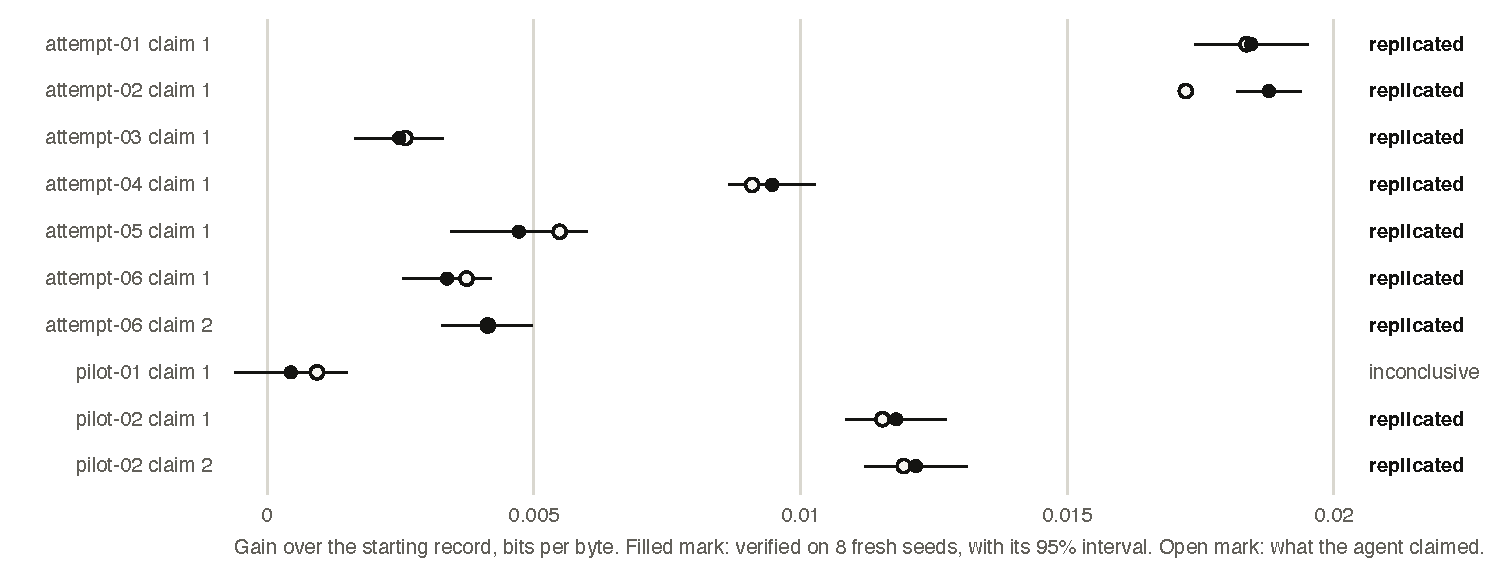
\includegraphics[width=\linewidth]{fig/claims.pdf}
\caption{Claimed and verified gain for each claim, pilots included and labeled.}\label{fig:claims}
\end{figure}

\paragraph{Fresh windows.} Every score reads the same 1024 windows, so every interval covers seed noise on those windows only. Each record from \vfreshfirst{} on was rescored on the next 1024 test windows, which no score had read, on 8 new seeds (Table~\ref{tab:fresh}). The gain to the current record is \vfreshusedgain{} bits per byte on the usual windows and \vfreshfreshgain{} on the new ones, and for the last record alone \vfreshlastused{} and \vfreshlastfresh{}.

\begin{table}[h]\centering\small
\begin{tabular}{lccc}
\toprule
Record & Usual 1024 windows & Next 1024 windows & Difference \\
\midrule
\bottomrule
\end{tabular}

\caption{Mean bits per byte over 8 seeds. One trained model per seed reads both sets of windows.}\label{tab:fresh}
\end{table}

\paragraph{Null control.} Each starting record went through the same pipeline unchanged, 8 times with 8 seeds each. That gave \vnullfalse{} false positives in \vnulln{} runs across \vnullrecords{} records, and 8 nulls per record can only catch a broken pipeline. \vnullrefuted{} run came back refuted, on a record whose stored batch sits about 2.1 standard errors below the mean of its nulls. This is the shared comparison batch limit named in the plan, and it means gains measured against that record read about 0.0005 low.

\paragraph{What bought the gains.} No agent replaced the model. Hashed context mixing in the PAQ tradition \cite{paq} was already the best recipe at this budget, and each agent record works inside it, by fixing a padding artefact at the start of a window, replacing hand-set constants with a learned gate, adding word contexts, fitting that gate on fresh bytes, or thinning high-order tables. Fresh Claude reviewers derived the mechanism of each record from its logs, and much of the gain is tied to this track. A review can refuse a record, but none has. About a third of record 07's gain (0.0061 of 0.0187, one seed, dev) sits in the first 16 of 512 positions of a window, and about three quarters of the gain in attempt-04's record 09 is eval-time modelling, paid for with 36.5\% more eval ticks. Passing the record rule does not show that a gain generalizes or that the agent understood it. One review found an agent's explanation only half right, and another found an agent crediting a change that cost ticks, where dropping stages was what paid for the gain.

\section{Related work}
The single \texttt{train.py} and the bits-per-byte framing come from karpathy/autoresearch. modded-nanogpt and Parameter Golf set the pattern of statistical record rules, with submitter-run logs, and Prime Intellect's autonomous speedrun has agents face a frozen verifier on eight fixed seeds. odometer differs in that the verifier draws fresh seeds and runs the test against the incumbent's stored seeds, on hardware the reader owns. The survival of agent claims has been measured before, in a nanoGPT setting where 8 of 15 non-null candidates replicated on sealed seeds \cite{lucky}, and the winner's curse has been measured for prompt-level self-improvement \cite{curse}. A recent audit of performance benchmarks shows how fragile wall-clock scoring is across machine types \cite{perfaudit}. The nearest precedent I know of is ARC's White-Box Estimation Challenge \cite{arc}, whose public leaderboard ranks estimators on FLOPs counted per operation from tensor shapes and dtypes, so that an estimator reads the same count on a laptop and on the grader. It meters estimation on random networks and not a training run. Green AI \cite{greenai} proposed operation counts as a hardware-independent measure of work, and the MicroNet Challenge \cite{micronet} scored inference that way. I found no public record track that meters the training run itself, from about a dozen searches, which is not proof.

\section{Limits}
The series measures one model, one prompt and one allowance on one corpus and one budget, with \vattempts{} attempts, so the interval is wide and it says nothing about agents in general. At a seed standard deviation of 0.001 the record rule passes a true gain of 0.003 about \vruleOOO{} of the time and 0.004 about \vruleOOF{}, and the weaker \emph{replicated} test passes one standard deviation about \vreppower{} of the time. The recipes were ported and tuned with a coding agent, and the reviews that decide a record come from fresh Claude sessions, not from human experts. No person has run the track, so nothing here compares agents with people.

\paragraph{Disclosure.} This project was built with Claude Code under my direction, including the engine, the verifier, the recipes, the harness and drafts of this text. I am responsible for its claims. Code, logs, transcripts and every number's command are in the repository, and \texttt{python reproduce.py} reruns the current record from a clean clone.

\begin{thebibliography}{12}\small
\bibitem{arc} J.~Hilton, P.~Christiano and collaborators. Announcing the ARC White-Box Estimation Challenge, 2026. \url{https://www.lesswrong.com/posts/Kben8CzS4awCwNw5c}
\bibitem{greenai} R.~Schwartz, J.~Dodge, N.~A.~Smith and O.~Etzioni. Green AI. arXiv:1907.10597, 2019.
\bibitem{micronet} MicroNet Challenge, 2019. \url{https://micronet-challenge.github.io/scoring_and_submission}
\bibitem{tinystories} R.~Eldan and Y.~Li. TinyStories: how small can language models be and still speak coherent English? arXiv:2305.07759, 2023.
\bibitem{paq} M.~Mahoney. Adaptive weighing of context models for lossless data compression. Florida Tech. Technical Report CS-2005-16, 2005.
\bibitem{lucky} Separating real improvements from lucky runs in autonomous ML research. NeurIPS 2026 Workshop for Autonomous Machine Learning Research (poster). \url{https://neurips.cc/virtual/2026/157611}
\bibitem{curse} L.~Hu and Y.~Tang. The winner's curse in LLM self-improvement loops: selection noise, lock-in, and acceptance rules. arXiv:2610.09239, 2026.
\bibitem{perfaudit} Z.~Chen, Z.~Sun, Y.~Shi, D.~Lo and L.~Jiang. Are performance-optimization benchmarks reliably measuring coding agents? arXiv:2607.01211, 2026.
\end{thebibliography}
\end{document}
